\documentclass{article}
\usepackage{polski} %moze wymagac dokonfigurowania latexa, ale jest lepszy niż standardowy babel'owy [polish]
\usepackage[utf8]{inputenc}
\usepackage[OT4]{fontenc}
\usepackage{amstext,subcaption,graphicx,color} %include pdf's (and png's for raster graphics... avoid raster graphics!)
\usepackage{url}
\usepackage[pdftex,hyperfootnotes=false,pdfborder={0 0 0}]{hyperref} %za wszystkimi pakietami; pdfborder nie wszedzie tak samo zaimplementowane bo specyfikacja nieprecyzyjna; pod miktex'em po prostu nie widac wtedy ramek
\let\myBib\thebibliography
\let\endmyBib\endthebibliography

\renewcommand\thebibliography[1]{\ifx\relax#1\relax\else\myBib{#1}\fi}

% Zmiana rozmiarów strony tekstu
\addtolength{\voffset}{-1cm}
\addtolength{\hoffset}{-1cm}
\addtolength{\textwidth}{2cm}
\addtolength{\textheight}{2cm}

%bardziej zyciowe parametry sterujace rozmieszczeniem rysunkow
\renewcommand{\topfraction}{.85}
\renewcommand{\bottomfraction}{.7}
\renewcommand{\textfraction}{.15}
\renewcommand{\floatpagefraction}{.66}
\renewcommand{\dbltopfraction}{.66}
\renewcommand{\dblfloatpagefraction}{.66}
\setcounter{topnumber}{9}
\setcounter{bottomnumber}{9}
\setcounter{totalnumber}{20}
\setcounter{dbltopnumber}{9}

% własny bullet list z malymi odstepami
\newenvironment{tightlist}{
\begin{itemize}
  \setlength{\itemsep}{1pt}
  \setlength{\parskip}{0pt}
  \setlength{\parsep}{0pt}}
{\end{itemize}}

%obrazkow szukamy w nastepujacym katalogu:
\graphicspath{{pics/}}



\begin{document}

\thispagestyle{empty} %bez numeru strony

\begin{center}
{\large{Sprawozdanie z laboratorium:\\
Komunikacja człowiek-komputer\\
}}

\vspace{3ex}

Część I: Python i wizualizacja

\vspace{3ex}
{\footnotesize\today}

\end{center}


\vspace{10ex}

Prowadzący: dr hab.~inż. Maciej Komosiński

\vspace{5ex}

Autor:
\begin{tabular}{lllr}
\textbf{Michał Lewiński} & inf122505 & WI & michal.lewinski@student.put.poznan.pl \\
\end{tabular}

\vspace{5ex}

Zajęcia środowe, 16:50.

\vspace{35ex}

\noindent Oświadczam/y, że niniejsze sprawozdanie zostało przygotowane wyłącznie przez powyższych autora/ów,
a wszystkie elementy pochodzące z innych źródeł zostały odpowiednio zaznaczone i~są cytowane w bibliografii.

\newpage


\section{Wstęp}
Zadanie laboratoryjne polegało na zapoznaniu się z różnymi metodami przekształcania obrazu oraz znalezienia krawędzi obiektów na obrazie. Do obsługi obrazu posłużono się biblioteką \textit{scikit-image}.
\section{Mozaika samolotów}
\begin{figure}
\begin{center}
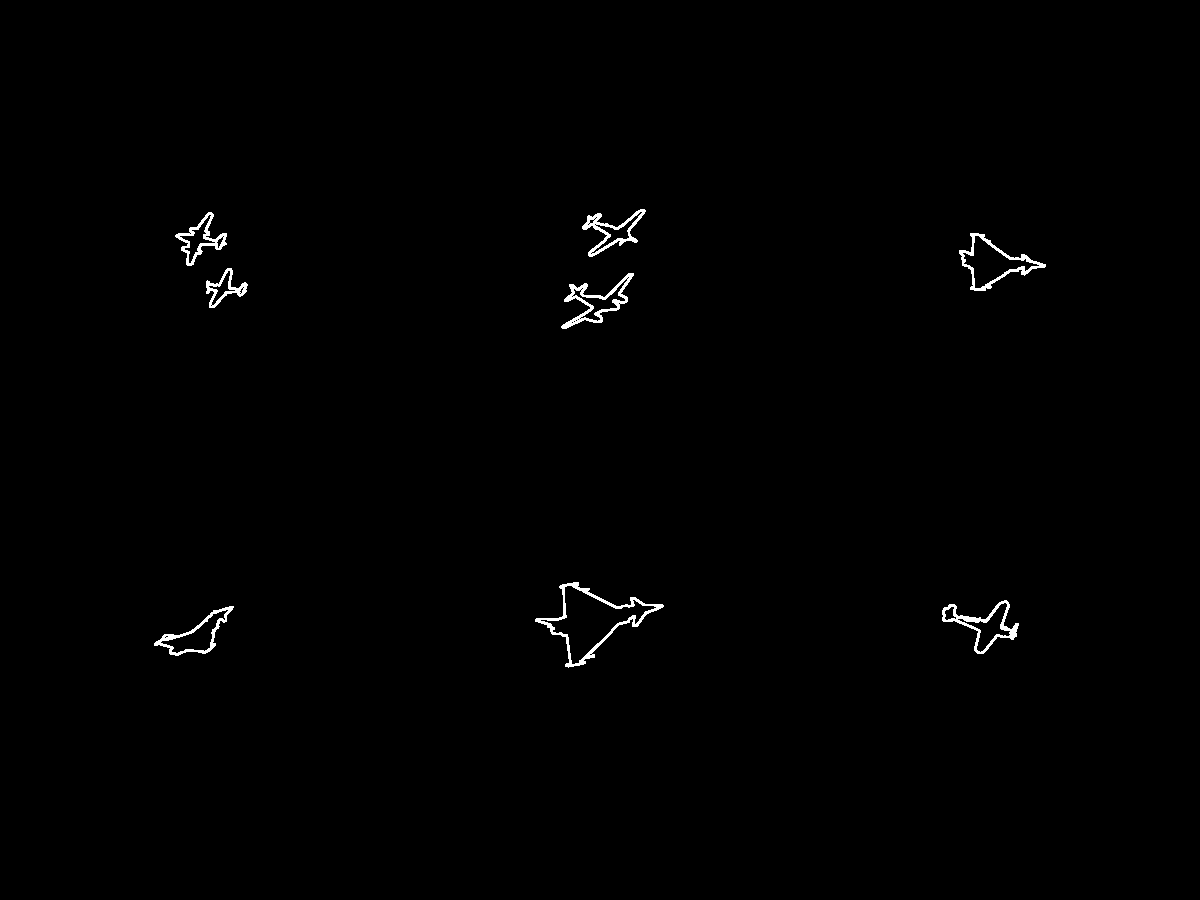
\includegraphics[width=1.0\textwidth]{samoloty.pdf}
\end{center}
\caption{Mozaika 6 obrazów, przedstawiających kontury różnych samolotów}
\label{fig:samoloty}
\end{figure}
Celem ćwiczenia było utworzenie mozaiki 6 obrazów, które przedstawiałyby tylko białe kontury samolotów na czarnym tle. Aby uzyskać kontury posłużono się odpowiednimi przekształceniami, które pozwoliły w sposób ogólny (nie zależny od obrazu) znaleźć krawędzie szukanych obiektów. Algorytm tworzenia mozaiki przedstawia się następująco:
\begin{enumerate}
\item Wczytanie pliku obrazu do macierzy z wartościami (R,G,B), za pomocą funkcji \textit{imread}~\cite{imread}.
\item Utworzenie osobnego subplotu dla obrazu.
\item Zwiększenie kontrastu obrazu za pomocą tzw. ,,contrast stretching", gdzie obraz jest przeskalowany, w taki sposób aby zawierał wszystkie wartości, które przypadają pomiędzy dwoma podanymi percentylami (w tym przypadku 1 i 20)~\cite{kontrast}.
\item Następnie dochodzi do konwersacji z przestrzeni \textit{RGB} do przestrzeni \textit{HSV}, gdyż potrzebujemy tylko wartości \textit{V}.
\item Na podstawie wartości \textit{V} i przy użyciu funkcji \textit{find\_contours} znajdujemy krawędzie obiektów. Funkcja ta wykorzystuję algorytm ,,marching squares" i zwraca listę odszukanych krawędzi, które są następnie wykorzystywane przy rysowaniu konturów~\cite{kontury}. 
\end{enumerate}

\bibliographystyle{unsrt} 
\bibliography{sprawozd}{}

\end{document}
